% answers.tex —— 2017 年·全国Ⅱ卷·文科 · 参考答案与详细解析片段
% 由 tools/generate_projects.py 依来源总账自 2017/2017_数学真题_全国2文_试题.md + 2017/2017_数学真题_全国2文_解析正文.md + 2017/2017_数学真题_全国2文_答案要点.md 生成，勿手改（改源 MD 后重跑）


\begin{gknotice}
\textbf{解析归属}：题面来源不附答案。以下推导由本库独立完成并经另一角色盲核；非官方解析。第 17(2) 题保留原题允许的两个分支。
\end{gknotice}

\begin{answer}
\gksolhead{1}{}

\textbf{题目}：

设集合 \(A=\{1,2,3\}\)，\(B=\{2,3,4\}\)，则 \(A\cup B=\)（　）

（A）\(\{1,2,3,4\}\)　（B）\(\{1,2,3\}\)　（C）\(\{2,3,4\}\)　（D）\(\{1,3,4\}\)

\Needspace{4\baselineskip}
\textbf{解析}

并集包含两个集合出现过的全部元素，合并并去重后为 \(\{1,2,3,4\}\)。

\gkanswer{答案：A（D）}

\end{answer}
\begin{answer}
\gksolhead{2}{}

\textbf{题目}：

\((1+i)(2+i)=\)（　）

（A）\(1-i\)　（B）\(1+3i\)　（C）\(3+i\)　（D）\(3+3i\)

\Needspace{4\baselineskip}
\textbf{解析}

展开得 \((1+\mathrm i)(2+\mathrm i)=2+3\mathrm i+\mathrm i^2=1+3\mathrm i\)。

\gkanswer{答案：B（D）}

\end{answer}
\begin{answer}
\gksolhead{3}{}

\textbf{题目}：

函数 \(f(x)=\sin\left(2x+\dfrac{\pi}{3}\right)\) 的最小正周期为（　）

（A）\(4\pi\)　（B）\(2\pi\)　（C）\(\pi\)　（D）\(\dfrac{\pi}{2}\)

\Needspace{4\baselineskip}
\textbf{解析}

正弦函数的角频率为 \(2\)，故最小正周期为 \(2\pi/2=\pi\)。

\gkanswer{答案：C（D）}

\end{answer}
\begin{answer}
\gksolhead{4}{}

\textbf{题目}：

设非零向量 \(\boldsymbol a,\boldsymbol b\) 满足 \(|\boldsymbol a+\boldsymbol b|=|\boldsymbol a-\boldsymbol b|\)，则（　）

（A）\(\boldsymbol a\perp\boldsymbol b\)　（B）\(|\boldsymbol a|=|\boldsymbol b|\)　（C）\(\boldsymbol a\parallel\boldsymbol b\)　（D）\(|\boldsymbol a|>|\boldsymbol b|\)

\Needspace{4\baselineskip}
\textbf{解析}

将模长等式平方并展开，两边相减得 \(4\boldsymbol a\cdot\boldsymbol b=0\)，故两向量垂直。

\gkanswer{答案：A（D）}

\end{answer}
\begin{answer}
\gksolhead{5}{}

\textbf{题目}：

若 \(a>1\)，则双曲线 \(\dfrac{x^2}{a^2}-y^2=1\) 的离心率的取值范围是（　）

（A）\((\sqrt2,+\infty)\)　（B）\((\sqrt2,2)\)　（C）\((1,\sqrt2)\)　（D）\((1,2)\)

\Needspace{4\baselineskip}
\textbf{解析}

双曲线的离心率为 \(e=\sqrt{a^2+1}/a=\sqrt{1+1/a^2}\)。由 \(a>1\) 得 \(1<e<\sqrt2\)。

\gkanswer{答案：C（D）}

\end{answer}
\begin{answer}
\gksolhead{6}{}

\textbf{题目}：

如图，网格纸上小正方形的边长为 \(1\)，粗实线画出的是某几何体的三视图，该几何体由一平面将一圆柱截去一部分后所得，则该几何体的体积为（　）
\nopagebreak[4]
\begin{center}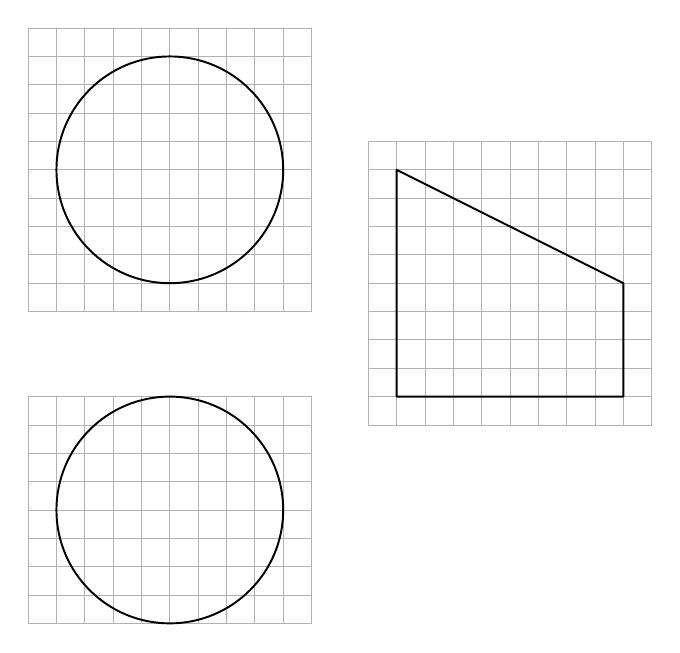
\begin{tikzpicture}[line cap=round,line join=round,line width=0.7pt,scale=0.36]
\begin{scope}[shift={(0,11)}]
  \draw[gray!60,line width=0.3pt] (0,0) grid (10,10);
  \draw (5,5) circle (4);
\end{scope}
\begin{scope}[shift={(12,7)}]
  \draw[gray!60,line width=0.3pt] (0,0) grid (10,10);
  \draw (1,1)--(9,1)--(9,5)--(1,9)--cycle;
\end{scope}
\begin{scope}
  \draw[gray!60,line width=0.3pt] (0,0) grid (10,8);
  \draw (5,4) circle (4);
\end{scope}
\end{tikzpicture}
\end{center}
\nopagebreak[4]
（A）\(90\pi\)　（B）\(63\pi\)　（C）\(42\pi\)　（D）\(36\pi\)

\Needspace{4\baselineskip}
\textbf{解析}

网格给出圆柱底面半径 \(3\)，截切后轴向两端高度分别为 \(10\) 与 \(4\)。截面高度在圆盘上是线性函数，其关于圆心的线性变化项平均为零，平均高度为 \((10+4)/2=7\)，所以体积等于 \(\pi\cdot3^2\cdot7\)。

\gkanswer{答案：B（D）}

\end{answer}
\begin{answer}
\gksolhead{7}{}

\textbf{题目}：

\Needspace{5\baselineskip}
设 \(x,y\) 满足约束条件
\nopagebreak[4]
\[
\begin{cases}
2x+3y-3\le 0,\\
2x-3y+3\ge 0,\\
y+3\ge 0,
\end{cases}
\]
则 \(z=2x+y\) 的最小值是（　）

（A）\(-15\)　（B）\(-9\)　（C）\(1\)　（D）\(9\)

\Needspace{4\baselineskip}
\textbf{解析}

可行域顶点为 \((-6,-3),(0,1),(6,-3)\)。目标函数 \(2x+y\) 在这三点分别取 \(-15,1,9\)，最小值出现在左下顶点。

\gkanswer{答案：A（D）}

\end{answer}
\begin{answer}
\gksolhead{8}{}

\textbf{题目}：

函数 \(f(x)=\ln(x^2-2x-8)\) 的单调递增区间为（　）

（A）\((-\infty,-2)\)　（B）\((-\infty,1)\)　（C）\((1,+\infty)\)　（D）\((4,+\infty)\)

\Needspace{4\baselineskip}
\textbf{解析}

\Needspace{5\baselineskip}
定义域由 \((x-4)(x+2)>0\) 得 \(( -\infty,-2)\cup(4,+\infty)\)。导数为
\nopagebreak[4]
\[
f'(x)=\frac{2x-2}{x^2-2x-8}.
\]
分母在定义域内为正；分子在左支为负、右支为正，所以仅 \((4,+\infty)\) 是递增区间。

\gkanswer{答案：D（D）}

\end{answer}
\begin{answer}
\gksolhead{9}{}

\textbf{题目}：

甲、乙、丙、丁四位同学一起去向老师询问成语竞赛的成绩。老师说：你们四人中有2位优秀，2位良好，我现在给甲看乙、丙的成绩，给乙看丙的成绩，给丁看甲的成绩。看后甲对大家说：我还是不知道我的成绩。根据以上信息，则（　）

（A）乙可以知道四人的成绩　（B）丁可以知道四人的成绩　（C）乙、丁可以知道对方的成绩　（D）乙、丁可以知道自己的成绩

\Needspace{4\baselineskip}
\textbf{解析}

若乙、丙成绩相同，甲便可由“两位优秀、两位良好”确定自己的成绩；甲仍不知道，说明乙、丙一优一良。于是甲、丁也一优一良。乙看见丙、丁看见甲后，均能确定自己的成绩。

\gkanswer{答案：D（D）}

\end{answer}
\begin{answer}
\gksolhead{10}{}

\textbf{题目}：

执行如图的程序框图，如果输入的 \(a=-1\)，则输出的 \(S=\)（　）
\nopagebreak[4]
\begin{center}\begin{tikzpicture}[line width=0.75pt,line cap=round,line join=round,font=\small]
\node[draw,rounded corners,minimum width=1.35cm,minimum height=0.5cm] (start) at (0,0) {开始};
\node[draw,minimum width=2.2cm,minimum height=0.55cm] (input) at (0,-0.95) {输入 $a$};
\node[draw,minimum width=2.7cm,minimum height=0.55cm] (init) at (0,-1.9) {$S=0,\ K=1$};
\coordinate (dt) at (0,-2.6);
\coordinate (dr) at (1.9,-3.2);
\coordinate (db) at (0,-3.8);
\coordinate (dl) at (-1.9,-3.2);
\draw (dt)--(dr)--(db)--(dl)--cycle;
\node at (0,-3.2) {$K\le 6$};
\node[draw,minimum width=3.0cm,minimum height=0.55cm] (sum) at (0,-4.55) {$S=S+a\cdot K$};
\node[draw,minimum width=2.3cm,minimum height=0.55cm] (flip) at (0,-5.45) {$a=-a$};
\node[draw,minimum width=2.6cm,minimum height=0.55cm] (next) at (0,-6.35) {$K=K+1$};
\node[draw,minimum width=1.9cm,minimum height=0.55cm] (out) at (3.6,-3.2) {输出 $S$};
\node[draw,rounded corners,minimum width=1.35cm,minimum height=0.5cm] (end) at (3.6,-4.2) {结束};
\draw[->] (start)--(input);
\draw[->] (input)--(init);
\draw[->] (init)--(dt);
\draw[->] (db)--node[right]{是}(sum);
\draw[->] (sum)--(flip);
\draw[->] (flip)--(next);
\draw[->] (next.west)--(-2.65,-6.35)--(-2.65,-3.2)--(dl);
\draw[->] (dr)--node[above]{否}(out.west);
\draw[->] (out)--(end);
\end{tikzpicture}
\end{center}
\nopagebreak[4]
（A）\(2\)　（B）\(3\)　（C）\(4\)　（D）\(5\)

\Needspace{4\baselineskip}
\textbf{解析}

循环变量 \(K\) 依次为 \(1,2,\ldots,6\)，每轮把 \(aK\) 加入 \(S\) 后将 \(a\) 变号。因此累计项为 \(-1,2,-3,4,-5,6\)，求和即可。

\gkanswer{答案：B（D）}

\end{answer}
\begin{answer}
\gksolhead{11}{}

\textbf{题目}：

从分别写有1，2，3，4，5的5张卡片中随机抽取1张，放回后再随机抽取1张，则抽得的第一张卡片上的数大于第二张卡片上的数的概率为（　）

（A）\(\dfrac{1}{10}\)　（B）\(\dfrac{1}{5}\)　（C）\(\dfrac{3}{10}\)　（D）\(\dfrac{2}{5}\)

\Needspace{4\baselineskip}
\textbf{解析}

两次有放回抽取共有 \(25\) 个等可能有序结果。第一张大于第二张时，从五个数中任选两个即可唯一确定一对有利次序，共 \(\binom52=10\) 种。

\gkanswer{答案：D（D）}

\end{answer}
\begin{answer}
\gksolhead{12}{}

\textbf{题目}：

过抛物线 \(C:y^2=4x\) 的焦点 \(F\)，且斜率为 \(\sqrt3\) 的直线交 \(C\) 于点 \(M\)（\(M\) 在 \(x\) 轴上方），\(l\) 为 \(C\) 的准线，点 \(N\) 在 \(l\) 上，且 \(MN\perp l\)，则 \(M\) 到直线 \(NF\) 的距离为（　）

（A）\(\sqrt5\)　（B）\(2\sqrt2\)　（C）\(2\sqrt3\)　（D）\(3\sqrt3\)

\Needspace{4\baselineskip}
\textbf{解析}

焦点 \(F=(1,0)\)，准线 \(x=-1\)。过焦点的直线为 \(y=\sqrt3(x-1)\)，与抛物线联立并取上半平面的交点得 \(M=(3,2\sqrt3)\)，故 \(N=(-1,2\sqrt3)\)。直线 \(NF\) 的方程为 \(\sqrt3x+y-\sqrt3=0\)，用点到直线距离公式求距。

\gkanswer{答案：C（D）}

\end{answer}
\begin{answer}
\gksolhead{13}{}

\textbf{题目}：

函数 \(f(x)=2\cos x+\sin x\) 的最大值为\gkblank{}。

\Needspace{4\baselineskip}
\textbf{解析}

由柯西不等式，\(2\cos x+\sin x\leq\sqrt{2^2+1^2}\)，等号可取，故最大值为振幅 \(\sqrt5\)。

\gkanswer{答案：\(\sqrt5\)（D）}

\end{answer}
\begin{answer}
\gksolhead{14}{}

\textbf{题目}：

已知函数 \(f(x)\) 是定义在 \(\mathbb R\) 上的奇函数，当 \(x\in(-\infty,0)\) 时，\(f(x)=2x^3+x^2\)，则 \(f(2)=\)\gkblank{}。

\Needspace{4\baselineskip}
\textbf{解析}

奇函数满足 \(f(2)=-f(-2)\)。将 \(-2\) 代入给定多项式，得 \(f(-2)=-12\)。

\gkanswer{答案：\(12\)（D）}

\end{answer}
\begin{answer}
\gksolhead{15}{}

\textbf{题目}：

长方体的长、宽、高分别为3，2，1，其顶点都在球 \(O\) 的球面上，则球 \(O\) 的表面积为\gkblank{}。

\Needspace{4\baselineskip}
\textbf{解析}

外接球直径为长方体体对角线，故 \((2r)^2=3^2+2^2+1^2=14\)，球表面积为 \(4\pi r^2=14\pi\)。

\gkanswer{答案：\(14\pi\)（D）}

\end{answer}
\begin{answer}
\gksolhead{16}{}

\textbf{题目}：

\(\triangle ABC\) 的内角 \(A,B,C\) 的对边分别为 \(a,b,c\)，若 \(2b\cos B=a\cos C+c\cos A\)，则 \(B=\)\gkblank{}。

\Needspace{4\baselineskip}
\textbf{解析}

余弦定理可写成 \(a\cos C+c\cos A=b\)。结合正弦定理将题设两边同除以 \(2R\)，得到 \(2b\cos B=b\)。因 \(b>0\)，有 \(\cos B=1/2\)。

\gkanswer{答案：\(B=\dfrac\pi3\)（D）}

\end{answer}
\begin{answer}
\gksolhead{17}{}

\textbf{题目}：

已知等差数列 \(\{a_n\}\) 的前 \(n\) 项和为 \(S_n\)，等比数列 \(\{b_n\}\) 的前 \(n\) 项和为 \(T_n\)，\(a_1=-1,b_1=1,a_2+b_2=2\)。

（1） 若 \(a_3+b_3=5\)，求 \(\{b_n\}\) 的通项公式；

（2） 若 \(T_3=21\)，求 \(S_3\)。

\Needspace{4\baselineskip}
\textbf{解析}

\gksubpart{(1) 数列参数}

设等差公差为 \(d\)、等比公比为 \(q\)。由首两项关系得 \(d+q=3\)；再由第三项关系得 \(2d+q^2=6\)，联立为 \(q(q-2)=0\)。在公比按相邻项商定义、因此取非零的通常约定下，只取 \(q=2\)，从而 \(b_n=2^{n-1}\)。若采用允许零公比的递推式约定，\(q=0,d=3\) 也满足已印条件，故此约定须在答案中明示。

\gksubpart{(2) 前三项和}

由 \(T_3=1+q+q^2=21\) 得 \((q-4)(q+5)=0\)。两根均为非零公比，分别对应 \(d=-1\) 与 \(d=8\)，而 \(S_3=-3+3d=6-3q\)。因此两支结果都符合原题，没有印刷条件可排除其一。

\gkanswer{答案（1）：\(b_n=2^{n-1}\)（D）}

\gkanswer{答案（2）：U。}

\end{answer}
\begin{answer}
\gksolhead{18}{}

\textbf{题目}：

如图，四棱锥 \(P-ABCD\) 中，侧面 \(PAD\) 为等边三角形且垂直于底面 \(ABCD\)，\(AB=BC=\dfrac12 AD\)，\(\angle BAD=\angle ABC=90^\circ\)。
\nopagebreak[4]
\begin{center}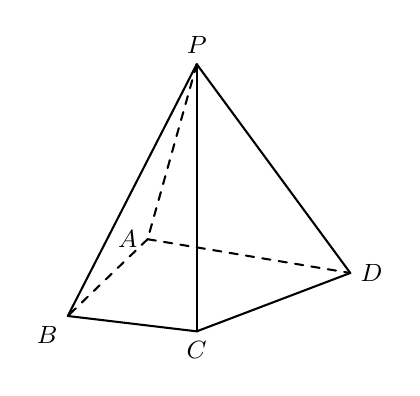
\begin{tikzpicture}[x=0.78cm,y=0.78cm,line cap=round,line join=round,line width=0.75pt,font=\small]
\coordinate (A) at (1.3,1.25);
\coordinate (B) at (0,0);
\coordinate (C) at (2.1,-0.25);
\coordinate (D) at (4.6,0.7);
\coordinate (P) at (2.1,4.1);
\draw (P)--(B)--(C)--(D)--(P);
\draw (P)--(C);
\draw[dashed] (P)--(A);
\draw[dashed] (A)--(B);
\draw[dashed] (A)--(D);
\node[above] at (P) {$P$};
\node[below left] at (B) {$B$};
\node[below] at (C) {$C$};
\node[right] at (D) {$D$};
\node[left] at (A) {$A$};
\end{tikzpicture}
\end{center}
\nopagebreak[4]
（1） 证明：直线 \(BC\parallel\) 平面 \(PAD\)；

（2） 若 \(\triangle PCD\) 面积为 \(2\sqrt7\)，求四棱锥 \(P-ABCD\) 的体积。

\Needspace{4\baselineskip}
\textbf{解析}

\gksubpart{(1) 线面平行}

底面中 \(BC\parallel AD\)，且 \(AD\subset\) 平面 \(PAD\)；\(BC\) 与平面 \(PAD\) 不重合，所以由线面平行判定定理，\(BC\parallel\) 平面 \(PAD\)。

\gksubpart{(2) 四棱锥体积}

令 \(AB=BC=x\)，则 \(AD=2x\)。以底面建立坐标，可取 \(A=(0,0,0),B=(0,x,0),D=(2x,0,0),C=(x,x,0),P=(x,0,\sqrt3x)\)。由题给三角形面积，\(|\overrightarrow{DP}\times\overrightarrow{DC}|/2=2\sqrt7\)，解得 \(x=2\)。底面为直角梯形，面积为 \(3x^2/2=6\)；锥高为 \(\sqrt3x=2\sqrt3\)，代入锥体积公式。

\gkanswer{答案（1）：\(BC\parallel\) 平面 \(PAD\)（D）}

\gkanswer{答案（2）：四棱锥体积 \(4\sqrt3\)（D）}

\end{answer}
\begin{answer}
\gksolhead{19}{}

\textbf{题目}：

海水养殖场进行某水产品的新、旧网箱养殖方法的产量对比，收获时各随机抽取了100个网箱，测量各箱水产品的产量（单位：kg），其频率分布直方图如图。
\nopagebreak[4]
\begin{center}\begin{tikzpicture}[x=0.68cm,y=0.68cm,line width=0.55pt,font=\scriptsize]
\begin{scope}
  \draw[->] (0,0)--(9.45,0);
  \draw[->] (0,0)--(0,7.55);
  \foreach \y/\lab/\x in {1.2/0.012/0,1.4/0.014/-1,2.0/0.020/0,2.4/0.024/0,3.2/0.032/0,3.4/0.034/-1,4.0/0.040/0} {
    \draw[densely dashed,gray] (0,\y)--(9,\y);
    \node[left] at (\x,\y) {\lab};
  }
  \foreach \x/\lab in {0/25,1/30,2/35,3/40,4/45,5/50,6/55,7/60,8/65,9/70} {
    \draw (\x,0)--(\x,-0.08);
    \node[below] at (\x,-0.12) {\lab};
  }
  \foreach \x/\h in {0/1.2,1/1.4,2/2.4,3/3.4,4/4.0,5/3.2,6/2.0,7/1.2,8/1.2} {
    \draw[fill=white] (\x,0) rectangle ++(1,\h);
  }
  \node[anchor=west] at (0.18,7.15) {频率/组距};
  \node at (4.5,-0.9) {箱产量/kg};
  \node at (4.5,-1.55) {旧养殖法};
\end{scope}
\begin{scope}[shift={(12,0)}]
  \draw[->] (0,0)--(7.45,0);
  \draw[->] (0,0)--(0,7.55);
  \foreach \y/\lab/\x in {0.4/0.004/0,0.8/0.008/-1,1.0/0.010/0,2.0/0.020/0,4.4/0.044/0,4.6/0.046/-1,6.8/0.068/0} {
    \draw[densely dashed,gray] (0,\y)--(7,\y);
    \node[left] at (\x,\y) {\lab};
  }
  \foreach \x/\lab in {0/35,1/40,2/45,3/50,4/55,5/60,6/65,7/70} {
    \draw (\x,0)--(\x,-0.08);
    \node[below] at (\x,-0.12) {\lab};
  }
  \foreach \x/\h in {0/0.4,1/2.0,2/4.4,3/6.8,4/4.6,5/1.0,6/0.8} {
    \draw[fill=white] (\x,0) rectangle ++(1,\h);
  }
  \node[anchor=west] at (0.18,7.15) {频率/组距};
  \node at (3.5,-0.9) {箱产量/kg};
  \node at (3.5,-1.55) {新养殖法};
\end{scope}
\end{tikzpicture}
\end{center}
\nopagebreak[4]
（1） 记 \(A\) 表示事件“旧养殖法的箱产量低于50 kg”，估计 \(A\) 的概率；

（2） 填写下面列联表，并根据列联表判断是否有99\%的把握认为箱产量与养殖方法有关；

\begin{center}
\begin{tabular}{lrr}
\toprule
 & 箱产量 < 50 kg & 箱产量 $\geq$ 50 kg \\
\midrule
旧养殖法 &  &  \\
新养殖法 &  &  \\
\bottomrule
\end{tabular}
\end{center}

（3） 根据箱产量的频率分布直方图，求新养殖法箱产量的优劣进行比较。

\Needspace{10\baselineskip}
附：

\begin{center}
\begin{tabular}{lrrr}
\toprule
\(P(K^2\ge k)\) & 0.050 & 0.010 & 0.001 \\
\midrule
\(K\) & 3.841 & 6.635 & 10.828 \\
\bottomrule
\end{tabular}
\end{center}

\nopagebreak[4]
\[
K^2=\frac{n(ad-bc)^2}{(a+b)(c+d)(a+c)(b+d)}.
\]

\Needspace{12\baselineskip}

\Needspace{4\baselineskip}
\textbf{解析}

\gksubpart{(1) 旧法低产概率}

\Needspace{5\baselineskip}
组距为 \(5\,\mathrm{kg}\)，频率等于柱高乘组距。旧法低于 \(50\,\mathrm{kg}\) 包括五组，累计频率为
\nopagebreak[4]
\[
5(0.012+0.014+0.024+0.034+0.040)=0.62.
\]

\gksubpart{(2) 独立性检验}

\Needspace{5\baselineskip}
将两组各 \(100\) 个网箱按 \(50\,\mathrm{kg}\) 分组，四格计数依次为旧法 \((62,38)\)、新法 \((34,66)\)。代入题给统计量：
\nopagebreak[4]
\[
K^2=\frac{200(62\cdot66-38\cdot34)^2}{100\cdot100\cdot96\cdot104}=\frac{1225}{78}\approx15.705.
\]
该值超过 99\% 对应的临界值 \(6.635\)。

\gksubpart{(3) 养殖效果比较}

按直方图组中值估算，旧法平均产量为 \(47.10\,\mathrm{kg}\)，新法为 \(52.35\,\mathrm{kg}\)；新法估计标准差约 \(6.30\,\mathrm{kg}\)，旧法约 \(10.36\,\mathrm{kg}\)。因此新法的估计产量较高且分布较集中。

\gkanswer{答案（1）：旧养殖法箱产量低于 \(50\,\mathrm{kg}\) 的估计概率为 \(0.62\)（D）}

\gkanswer{答案（2）：\(K^2=15.705>6.635\)，有 99\% 的把握认为箱产量与养殖方法有关（D）}

\gkanswer{答案（3）：新法估计平均产量 \(52.35\,\mathrm{kg}\)，旧法约 \(47.10\,\mathrm{kg}\)；新法分布更集中（估计标准差约 \(6.30\,\mathrm{kg}\)，旧法约 \(10.36\,\mathrm{kg}\)），故新法表现较优（D）。}

\end{answer}
\begin{answer}
\gksolhead{20}{}

\textbf{题目}：

设 \(O\) 为坐标原点，动点 \(M\) 在椭圆 \(C:\dfrac{x^2}{2}+y^2=1\) 上，过 \(M\) 作 \(x\) 轴的垂线，垂足为 \(N\)，点 \(P\) 满足 \(\overrightarrow{NP}=\sqrt2\,\overrightarrow{NM}\)。

（1） 求点 \(P\) 的轨迹方程；

（2） 设点 \(Q\) 在直线 \(x=-3\) 上，且 \(\overrightarrow{OP}\cdot\overrightarrow{PQ}=1\)。证明：过点 \(P\) 且垂直于 \(OQ\) 的直线 \(l\) 过 \(C\) 的左焦点 \(F\)。

\Needspace{4\baselineskip}
\textbf{解析}

\gksubpart{(1) 点的轨迹}

令 \(M=(u,v)\)，则垂足 \(N=(u,0)\)，向量条件给出 \(P=(u,\sqrt2v)\)。代入椭圆关系 \(u^2/2+v^2=1\)，得到 \(P\) 的坐标满足 \(x^2+y^2=2\)。

\gksubpart{(2) 垂线经过焦点}

\Needspace{5\baselineskip}
写 \(P=(x,y),Q=(-3,t)\)。由 \(x^2+y^2=2\) 及点积条件 \(\overrightarrow{OP}\cdot\overrightarrow{PQ}=1\)，化简得 \(yt=3(x+1)\)。左焦点为 \(F=(-1,0)\)，而
\nopagebreak[4]
\[
\overrightarrow{OQ}\cdot\overrightarrow{PF}=3(x+1)-yt=0.
\]
故 \(PF\perp OQ\)，所述过 \(P\) 的垂线通过 \(F\)。

\gkanswer{答案（1）：\(x^2+y^2=2\)（D）}

\gkanswer{答案（2）：所述过 \(P\) 且垂直于 \(OQ\) 的直线经过左焦点 \(F=(-1,0)\)（D）}

\end{answer}
\begin{answer}
\gksolhead{21}{}

\textbf{题目}：

设函数 \(f(x)=(1-x^2)e^x\)。

（1） 讨论 \(f(x)\) 的单调性；

（2） 当 \(x\ge0\) 时，\(f(x)\le ax+1\)，求 \(a\) 的取值范围。

\Needspace{4\baselineskip}
\textbf{解析}

\gksubpart{(1) 单调区间}

求导得 \(f'(x)=e^x(1-2x-x^2)\)。导数零点为 \(-1\pm\sqrt2\)，且指数因子恒正；二次因子在两根之间为正、两侧为负，据此判定三个单调区间。

\gksubpart{(2) 参数范围}

令 \(g(x)=x+1-f(x)\)。计算得 \(g(0)=g'(0)=0\)，且 \(g''(x)=(x^2+4x+1)e^x>0\)（\(x\ge0\)），所以 \(g(x)\ge0\)，即 \(f(x)\le x+1\)。这给出充分条件 \(a\ge1\)。若 \(a<1\)，则 \((f(x)-1)/x\to f'(0)=1\)（\(x\to0^+\)），足够小的正数会违反所需不等式，故没有更小的参数可行。

\gkanswer{答案（1）：\(f\) 在 \(( -\infty,-1-\sqrt2)\) 递减、\((-1-\sqrt2,-1+\sqrt2)\) 递增、\((-1+\sqrt2,+\infty)\) 递减（D）}

\gkanswer{答案（2）：\(a\in[1,+\infty)\)（D）}

\end{answer}
\begin{answer}
\gksolhead{22}{}

\textbf{题目}：

在直角坐标系 \(xOy\) 中，以坐标原点为极点，\(x\) 轴的正半轴为极轴建立极坐标系，曲线 \(C_1\) 的极坐标方程为 \(\rho\cos\theta=4\)。

（1） \(M\) 为曲线 \(C_1\) 上的动点，点 \(P\) 在线段 \(OM\) 上，且满足 \(|OM|\cdot|OP|=16\)，求点 \(P\) 的轨迹 \(C_2\) 的直角坐标方程；

（2） 设点 \(A\) 的极坐标为 \(\left(2,\dfrac{\pi}{3}\right)\)，点 \(B\) 在曲线 \(C_2\) 上，求 \(\triangle OAB\) 面积的最大值。

\Needspace{4\baselineskip}
\textbf{解析}

\gksubpart{(1) 轨迹方程}

极坐标条件表示直线 \(x=4\)。令 \(M=(4,t)\)，并写 \(P=\lambda M\)。由距离乘积得 \(\lambda=16/(16+t^2)\)，消去 \(t\) 后有 \(x^2+y^2=4x\)。有限 \(t\) 时 \(\lambda>0\)，原点不在实际轨迹中，故另有 \(x>0\) 的限制。

\gksubpart{(2) 面积最大值}

点 \(A=(1,\sqrt3)\)，轨迹圆心为 \((2,0)\)、半径为 \(2\)。三角形面积为 \(|\det(A,B)|/2\)；行列式在圆心处的常量项绝对值为 \(2\sqrt3\)，沿半径方向的最大变化量为 \(2|A|=4\)。极值点不为被排除的原点，故最大面积由 \((2\sqrt3+4)/2\) 取得。

\gkanswer{答案（1）：轨迹为 \(x^2+y^2=4x\) 且 \(x>0\)（圆周不含原点）（D）}

\gkanswer{答案（2）：三角形面积最大值为 \(2+\sqrt3\)（D）}

\end{answer}
\begin{answer}
\gksolhead{23}{}

\textbf{题目}：

已知 \(a>0,b>0,a^3+b^3=2\)，证明：

（1） \((a+b)(a^5+b^5)\ge4\)；

（2） \(a+b\le2\)。

\Needspace{4\baselineskip}
\textbf{解析}

\gksubpart{(1) 不等式}

\Needspace{5\baselineskip}
由恒等式
\nopagebreak[4]
\[
(a+b)(a^5+b^5)-(a^3+b^3)^2=ab(a^2-b^2)^2\ge0
\]
及 \(a^3+b^3=2\)，得到所需下界。

\gksubpart{(2) 不等式}

展开可得 \(4(a^3+b^3)-(a+b)^3=3(a+b)(a-b)^2\ge0\)。代入三次幂和条件并取正立方根，即得所需上界。

\gkanswer{答案（1）：\((a+b)(a^5+b^5)\ge4\)（D）}

\gkanswer{答案（2）：\(a+b\le2\)（D）}

\end{answer}